%%%%%%%%%%%%%%%%%%%%%%%%%%%%%%%%%%%%%%%%
% This template has been downloaded from https:overleaf.com/
% Licence: CC-BY
%%%%%%%%%%%%%%%%%%%%%%%%%%%%%%%%%%%%%%%%
\documentclass[12pt, letterpaper, oneside]{report}
\usepackage[lmargin=1in, rmargin=0.5in, tmargin=0.55in, bmargin=0.5in]{geometry}

\usepackage[english]{babel}
\usepackage[utf8]{inputenc}
%\usepackage{lipsum}
\usepackage{gensymb}
\usepackage{fancyhdr}


\usepackage{graphicx}   % Written by David Carlisle and Sebastian Rahtz
                        % Required if you want graphics, photos, etc.
                        % graphicx.sty is already installed on most LaTeX
                        % systems. The latest version and documentation can
                        % be obtained at:
                        % http://www.ctan.org/tex-archive/macros/latex/required/graphics/
                        % Another good source of documentation is "Using
                        % Imported Graphics in LaTeX2e" by Keith Reckdahl
                        % which can be found as esplatex.ps and epslatex.pdf
                        % at: http://www.ctan.org/tex-archive/info/

\usepackage{subcaption}
%\usepackage{psfrag}    % Written by Craig Barratt, Michael C. Grant,
                        % and David Carlisle
                        % This package allows you to substitute LaTeX
                        % commands for text in imported EPS graphic files.
                        % In this way, LaTeX symbols can be placed into
                        % graphics that have been generated by other
                        % applications. You must use latex->dvips->ps2pdf
                        % workflow (not direct pdf output from pdflatex) if
                        % you wish to use this capability because it works
                        % via some PostScript tricks. 


\usepackage{url}        % Written by Donald Arseneau
                        % Provides better support for handling and breaking
                        % URLs. url.sty is already installed on most LaTeX
                        % systems. The latest version can be obtained at:
                        % http://www.ctan.org/tex-archive/macros/latex/contrib/other/misc/
                        % Read the url.sty source comments for usage information.



\usepackage{amsmath}    % From the American Mathematical Society
                        % A popular package that provides many helpful commands
                        % for dealing with mathematics. Note that the AMSmath
                        % package sets \interdisplaylinepenalty to 10000 thus
                        % preventing page breaks from occurring within multiline
                        % equations. Use:


\usepackage{float}

\usepackage[toc,page]{appendix}
\pagestyle{fancy}
%\fancyhead[]

%%%%%%%%%%%%%%%%%%%%%%%%%%%%%%%%
%% Copyright (C) 2018 Almas Askarbekov.
%% License: CC-BY.
%% Share with attribution
%%%%%%%%%%%%%%%%%%%%%%%%%%%%%%%%
\begin{document}
\fancyhead[L]{\slshape \MakeUppercase Diamond section}
\fancyhead[R]{Almas Askarbekov}
\begin{titlepage}

\newcommand{\HRule}{\rule{\linewidth}{0.5mm}} % Defines a new command for the horizontal lines, change thickness here

\center % Center everything on the page
 
%----------------------------------------------------------------------------------------
%   HEADING SECTIONS
%----------------------------------------------------------------------------------------


%\textsc{\large Same problem, different angle}\\[0.5cm] 

%----------------------------------------------------------------------------------------
%   TITLE SECTION
%----------------------------------------------------------------------------------------

\HRule \\[0.8cm]
{ \huge \bfseries Diamond Section}\\[0.4cm] % Title of your document
{ \large \bfseries Doubling the cube. Solution.}\\[0.2cm]
\HRule \\[1.5cm]
\textsc{\large Same problem, different angle.}\\[0.5cm] 
%----------------------------------------------------------------------------------------
%   AUTHOR SECTION
%----------------------------------------------------------------------------------------

\begin{minipage}{0.8\textwidth}
\begin{center} \large


\end{center}

\begin{center}

\end{center}

\end{minipage}


\begin{figure}[h]
\centerline{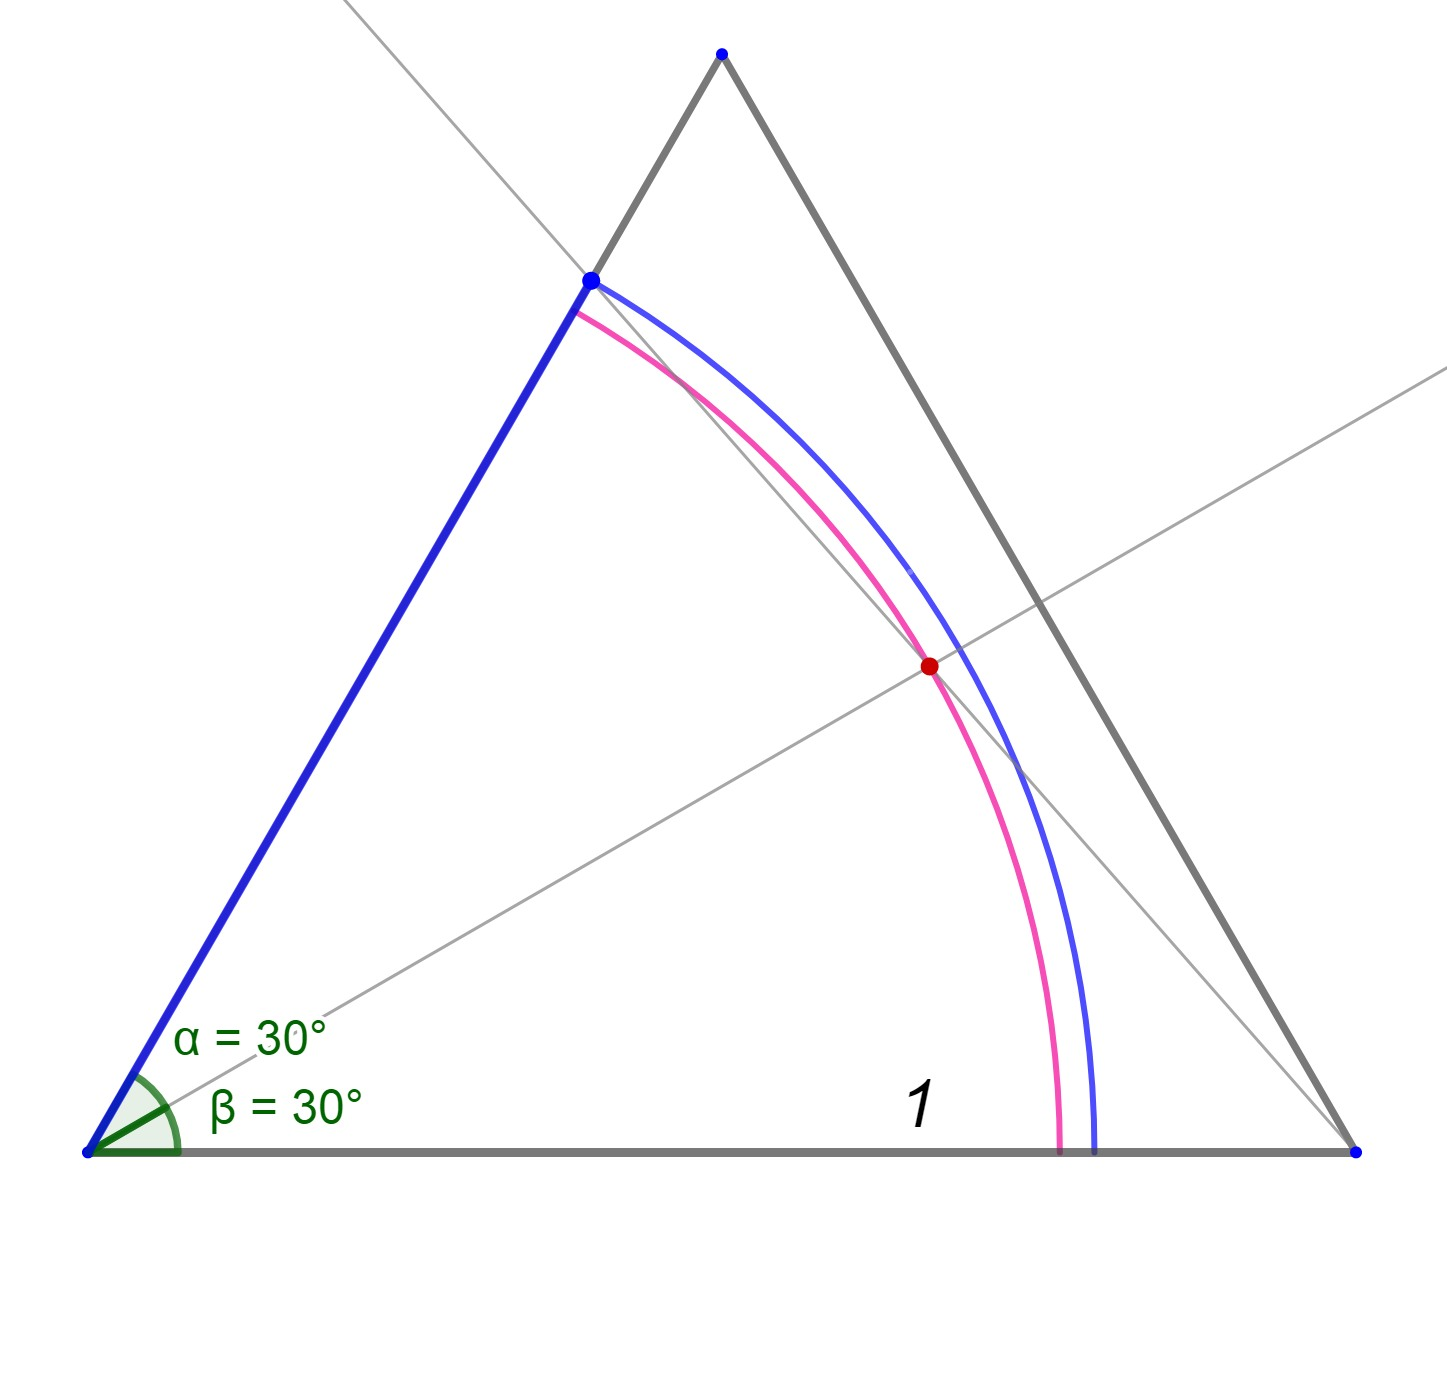
\includegraphics[scale=0.2]{ds_tr.jpg}}

\label{logo}
\end{figure}
\textsc{\LARGE Askarbekov Almas Serikovich }\\[1.5cm]
\begin{center}
	\large {jobspace@yandex.com}\\
	\today
\end{center}
\end{titlepage}


\begin{center}
\section*{Abstract}
\end{center}
Doubling the cube also known as the Delian problem is one of the three famous geometric problems of antiquity, unsolvable by compass and straightedge construction. Given the edge of a cube, the problem requires the construction of the edge of a second cube, whose volume is double that of the first.\\
\\
The only tools allowed for the construction is the unmarked straightedge and compass.\\
\\
In algebraic terms, doubling a unit cube requires the construction of a line segment of length x, where $x^{3} = 2$; in other words $x =\sqrt[3]{2}$.\\
Pierre Wantzel proved in 1837 that the $\sqrt[3]{2}$ can not be constructed with straightedge and compass.\cite{A} \\ 
\begin{figure}[h]
	\centering
	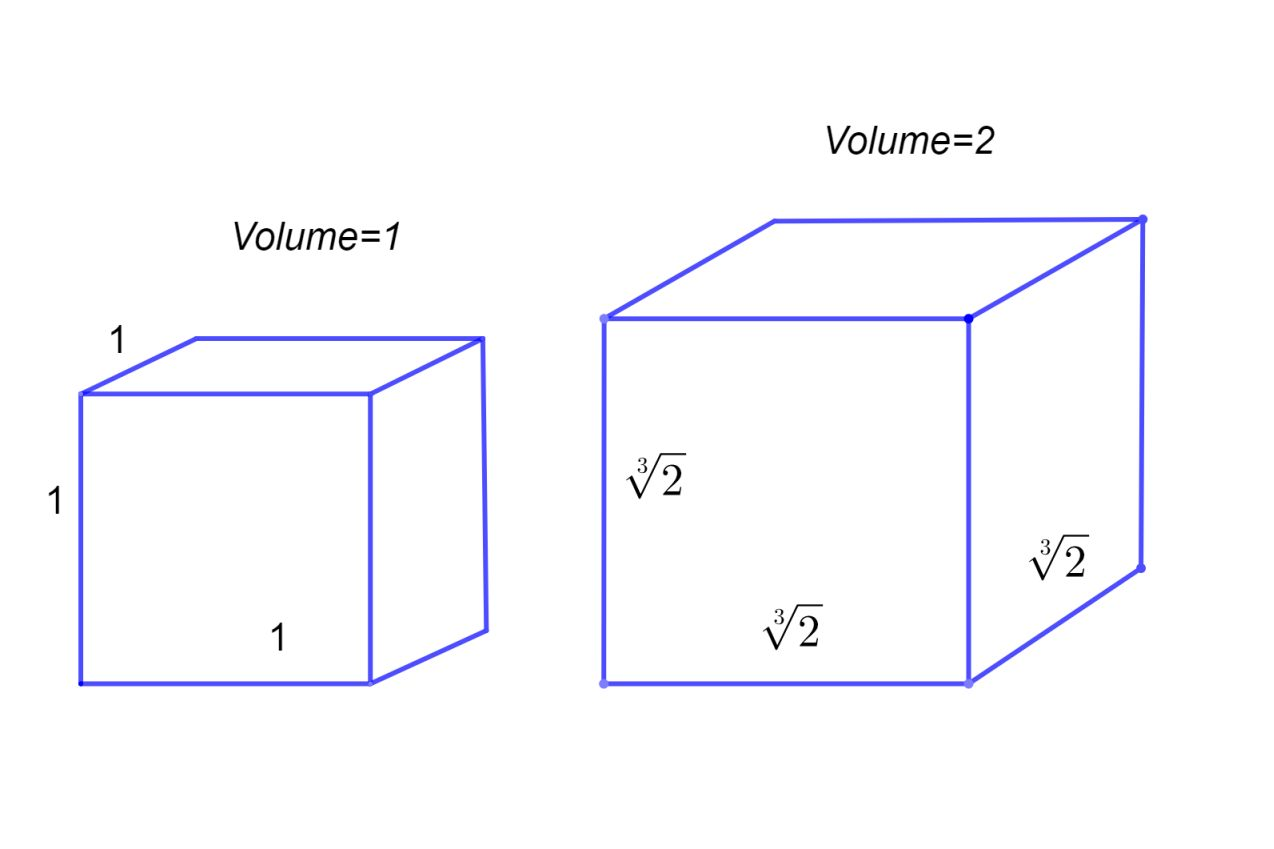
\includegraphics[width=0.7\linewidth]{cubes.jpg}
	\label{fig:cubes}
\end{figure}
\begin{figure}[h]
	\centering
	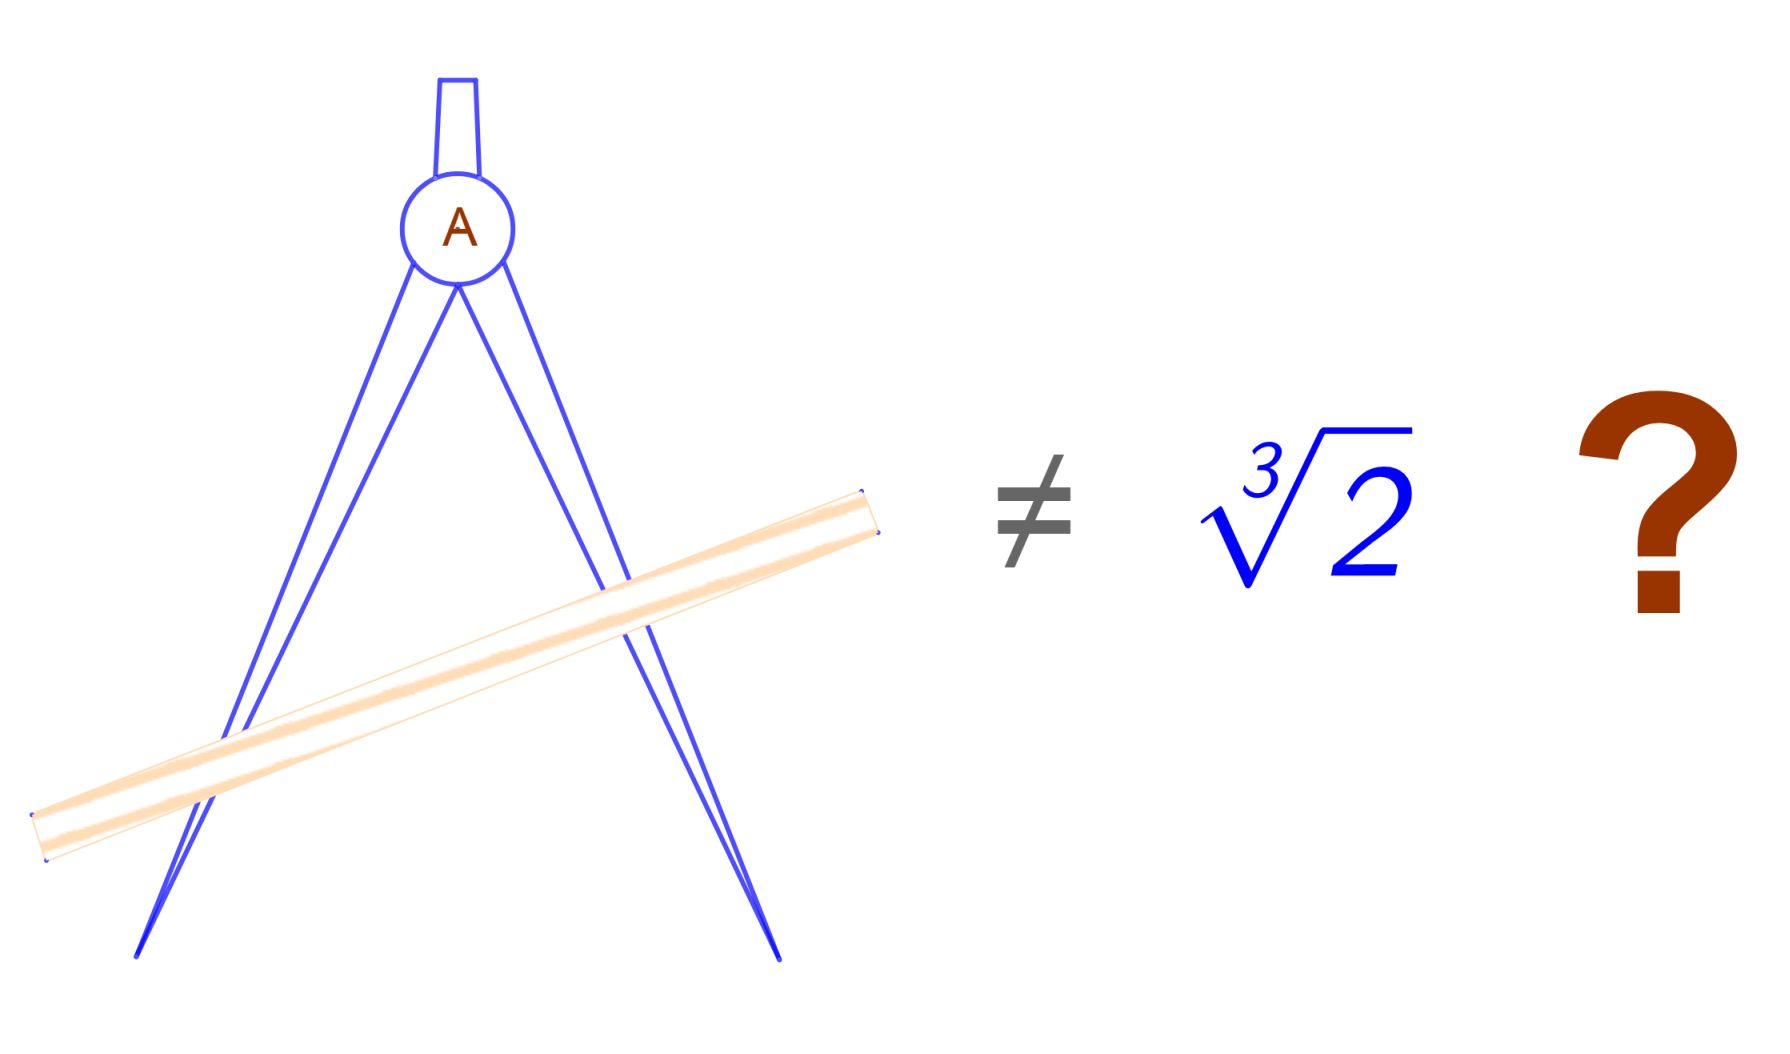
\includegraphics[width=0.8\linewidth]{compass.jpg}
	\label{fig:compass}
\end{figure}
\newpage

\tableofcontents


\chapter{The solution}

\section{Construction}
\begin{enumerate}
	\item Let's construct a sequence of circles as shown in Figure 1.1, with radius $r=1$.
\begin{figure}[H]
	\centerline{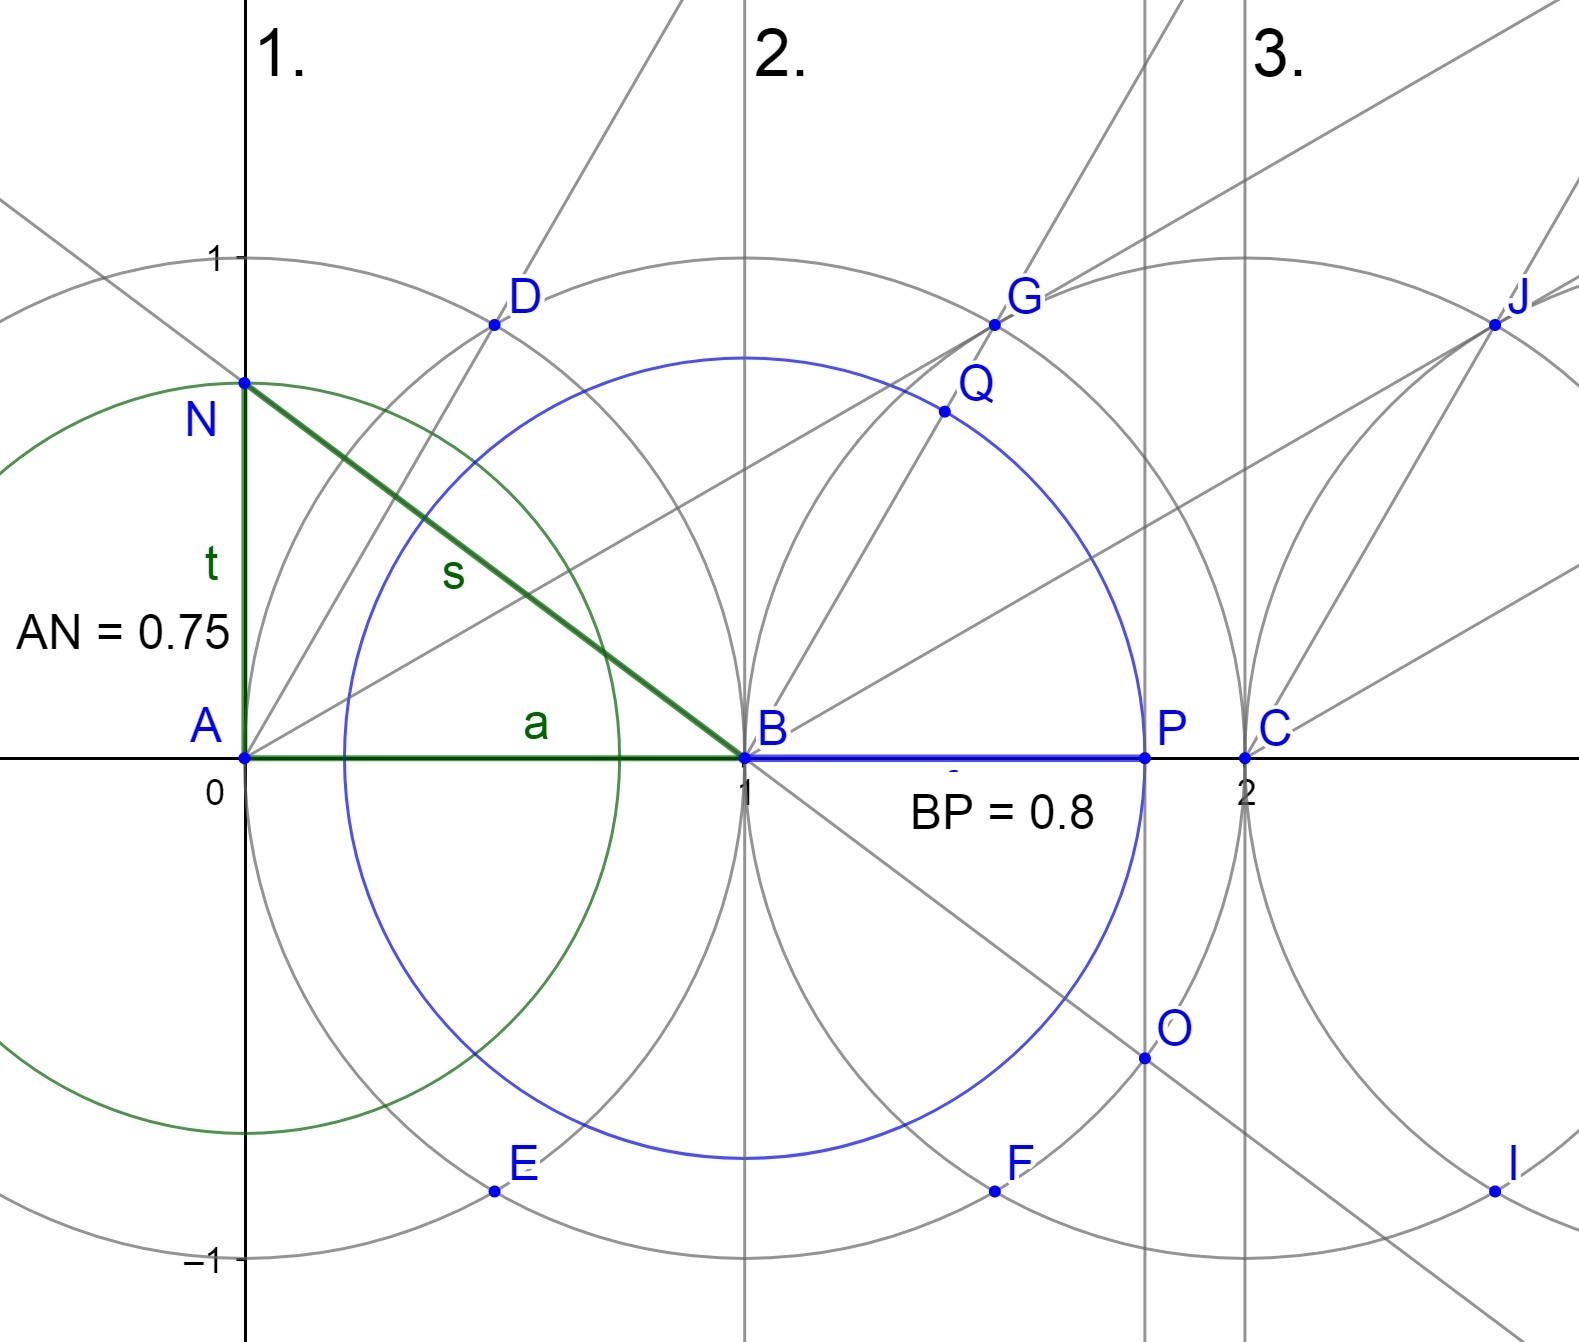
\includegraphics[scale=0.2]{secnd.jpg}}
	\caption{Basic circles and triangle}
	\label{fig:basic}
\end{figure}
	
	\item Then construct the right triangle $\triangle ANB$ (Figure \ref{fig:basic}) with shortest leg $t=0.75$. \\
	where:
\begin{equation}
s=\overline{NB}=\sqrt{a^{2}+t^{2}}=\sqrt{1^{2}+0.75^{2}}=1.25
\end{equation}
by the Pythagorean theorem. 
\begin{figure}[h]
	\centerline{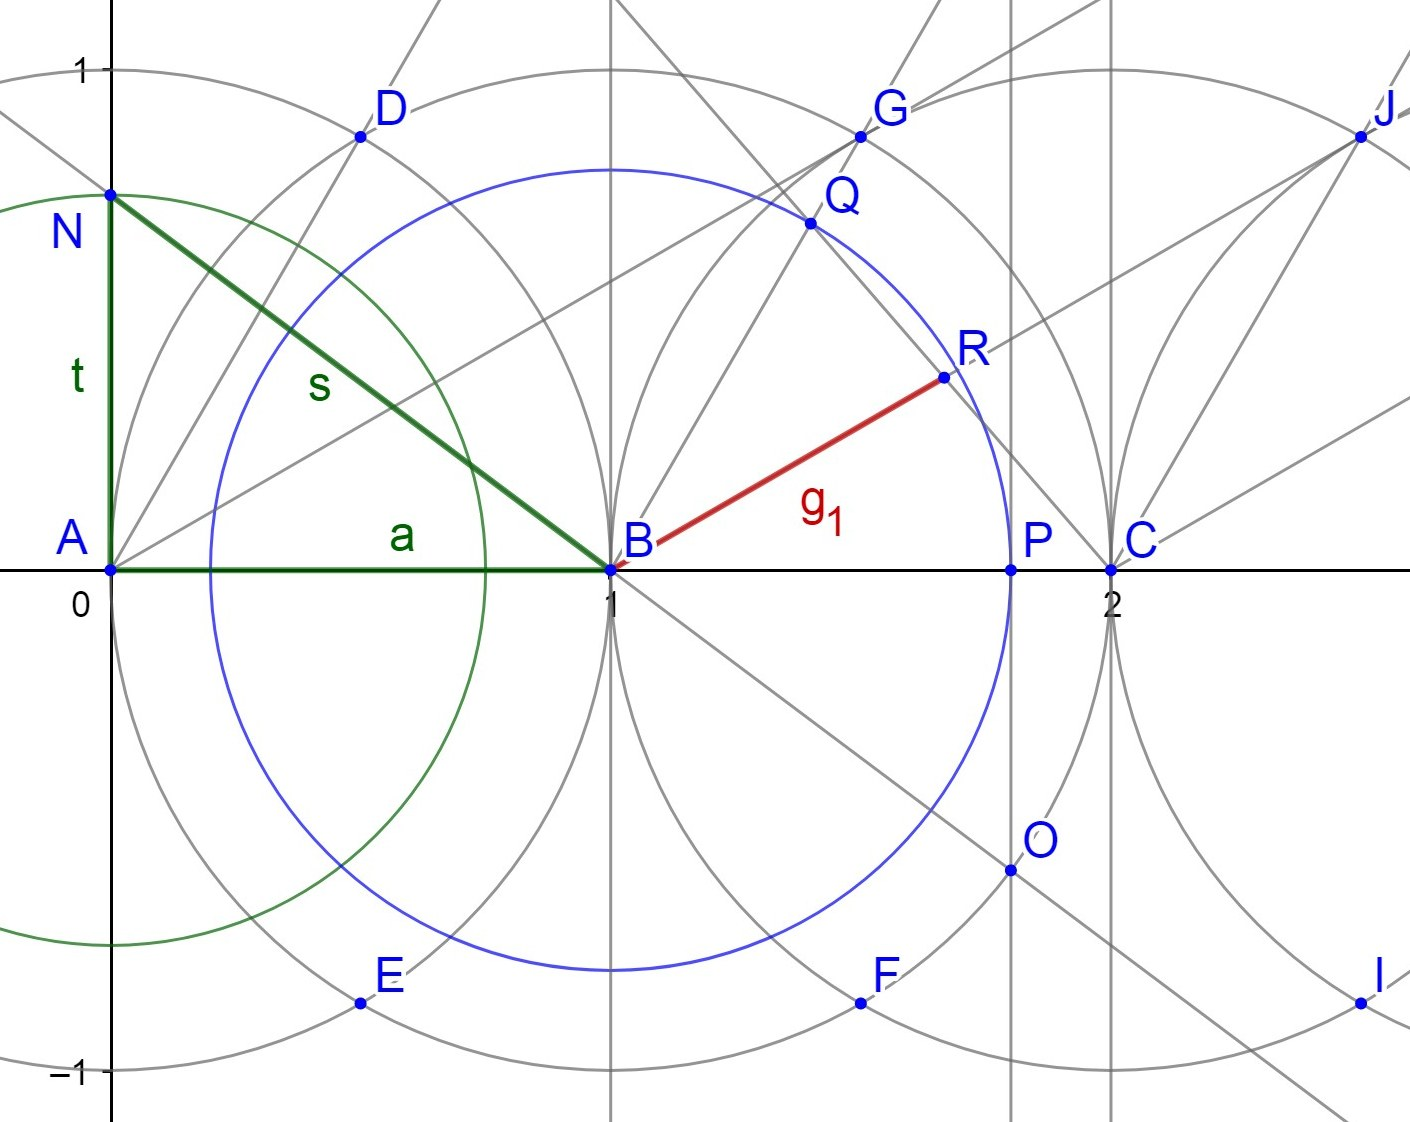
\includegraphics[scale=0.2]{intersection.jpg}}
	\caption{Intersection}
	\label{intersection}
\end{figure}
 
	\item Calculate cosine of $\angle ABN$:
\begin{equation}
	\dfrac{a}{s}=\dfrac{1}{1.25}=0.8.
\end{equation}
\newpage
To construct the ratio we obtain, we need to draw a line through $\overline{NB}$. Then we get the point $O$ as the intersection of the line and the circle with center at the point $B(1,0)$. So we get the line segment $BP=0.8$, as the projection of the point $O$ on the x-axis. (Figure \ref{intersection})\\ 
	
	\item Then construct a ray from point $C(2,0)$ through the intersection point $Q$ of the circle with radius $BP=0.8$ and the line segment $\overline{BG}$.
	\subitem Now we get the point $R$ and the line segment $\overline{BR}$. The segment $\overline{BR}$ is the bisector for $\triangle$ $CBQ$. (Figure 1.2)
	\item The \angle \textit{$\alpha$} of $\triangle$ $CBQ=\angle CBG=60\degree$, because $\triangle CBG$ is an equilateral triangle with sides equal to 1. (Figure \ref{fig:unit triangle})
\begin{figure}[H]
		\centerline{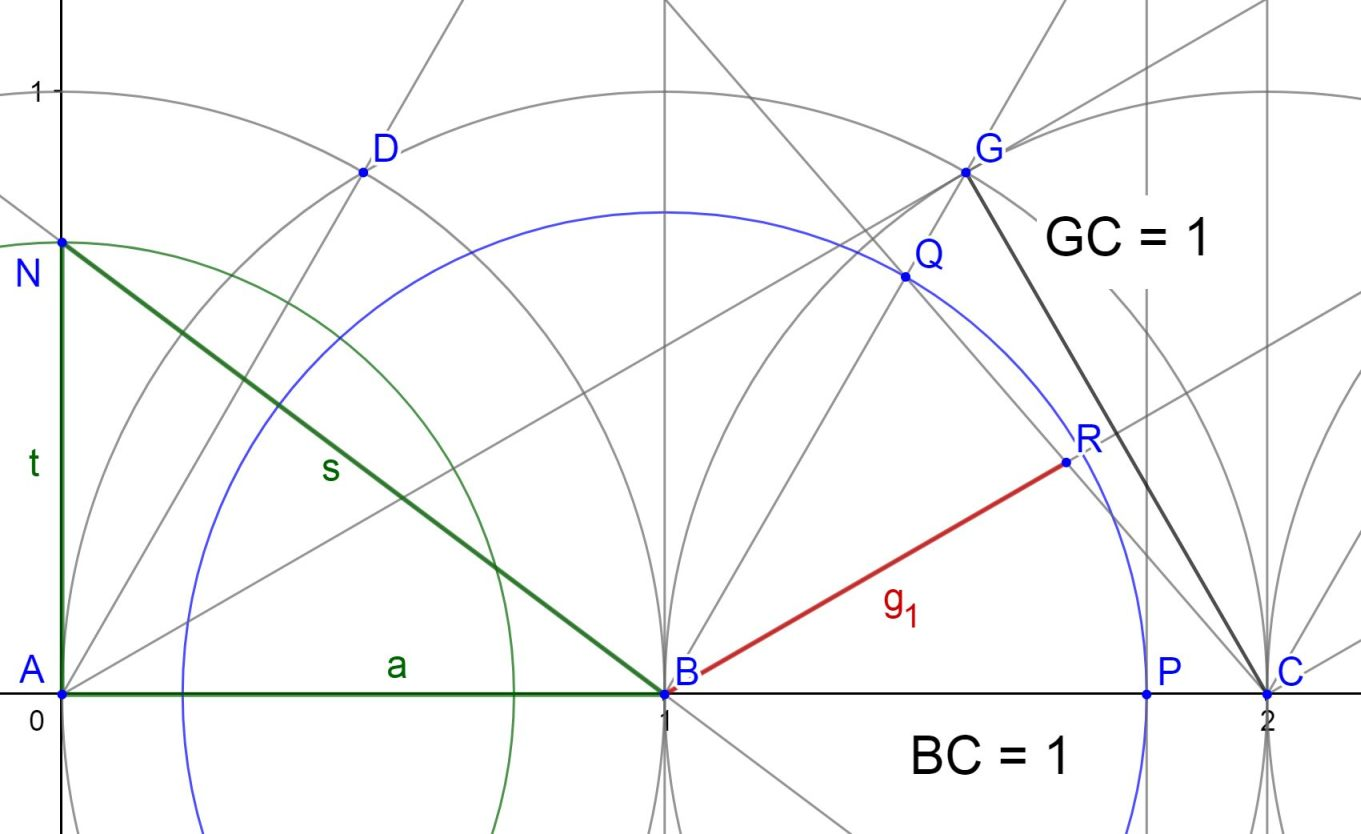
\includegraphics[scale=0.9]{cbg.jpg}}
		\caption{Equilateral triangle $CBG$}
		\label{fig:unit triangle}
\end{figure} 
\newpage
\begin{figure}[h]
	\centerline{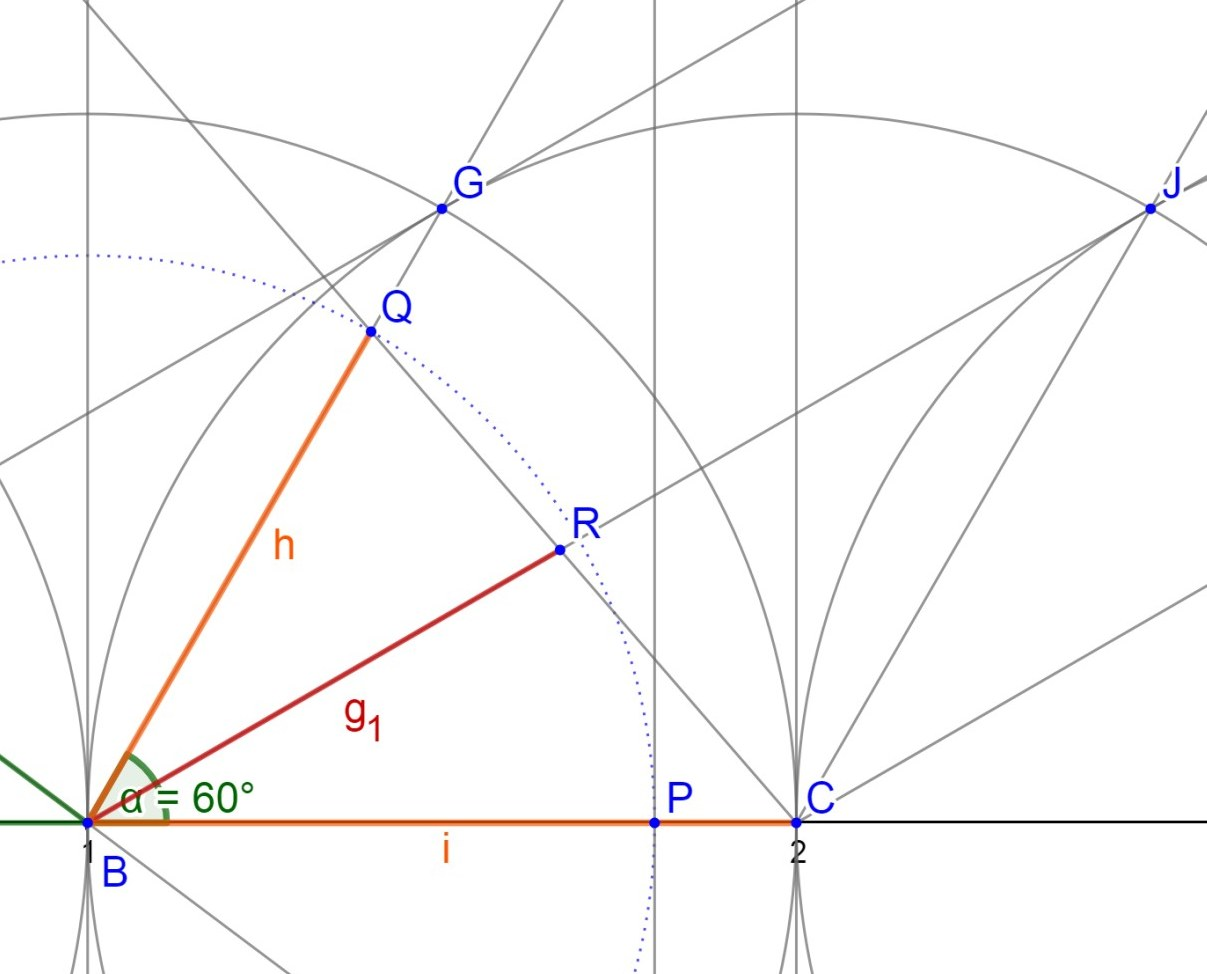
\includegraphics[scale=0.9]{bisector0.jpg}}
	\caption{Triangle bisector}
	\label{bisector}
\end{figure} 
	\item Let's calculate the length of the segment $\overline{BR}$ (Figure \ref{bisector}) by the formula for the 60 degree angle bisector\footnote{application of the law of cosines }:
\begin{equation}
		 g_{1}=\frac{2ih}{i+h}\times \cos 60\degree = \frac{2ih}{i+h}\times\frac{\sqrt{3}}{2}
\end{equation}.\\
	Where $h=\overline{BQ}=0.8$; $i=B,C=1$; therefore:
\begin{equation}	
g_{1}=\frac{2\times0.8}{1+0.8}\times\frac{\sqrt{3}}{2}\approx 0.769800358919501
\end{equation}.\\
	\item Now, let's draw a circle with radius $g_{1}$ with center at the point $B(1,0)$. Then we get the point $S$, as the intersection of the circle and the line perpendicular to x-axis through the point $B$. (Figure \ref{circle_r=bisector})
	 
\begin{figure}[h]
	\centerline{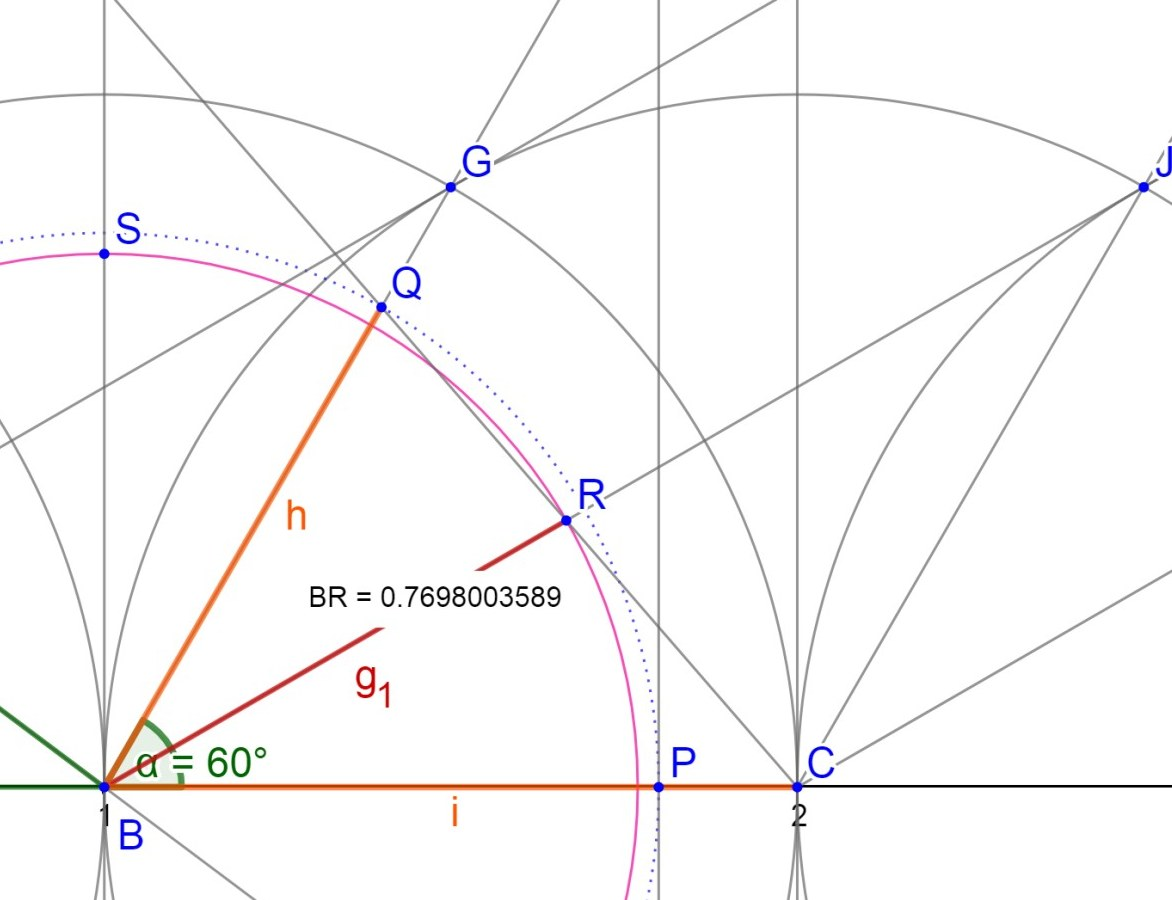
\includegraphics[scale=0.8]{circle.jpg}}
	\caption{Circle with radius = bisector $g_{1}$}
	\label{circle_r=bisector}
\end{figure}
\newpage
	\item Then construct the right triangle $\triangle CBS$ as shown in the Figure \ref{triangle_2}.
\begin{figure}[h]
	\centerline{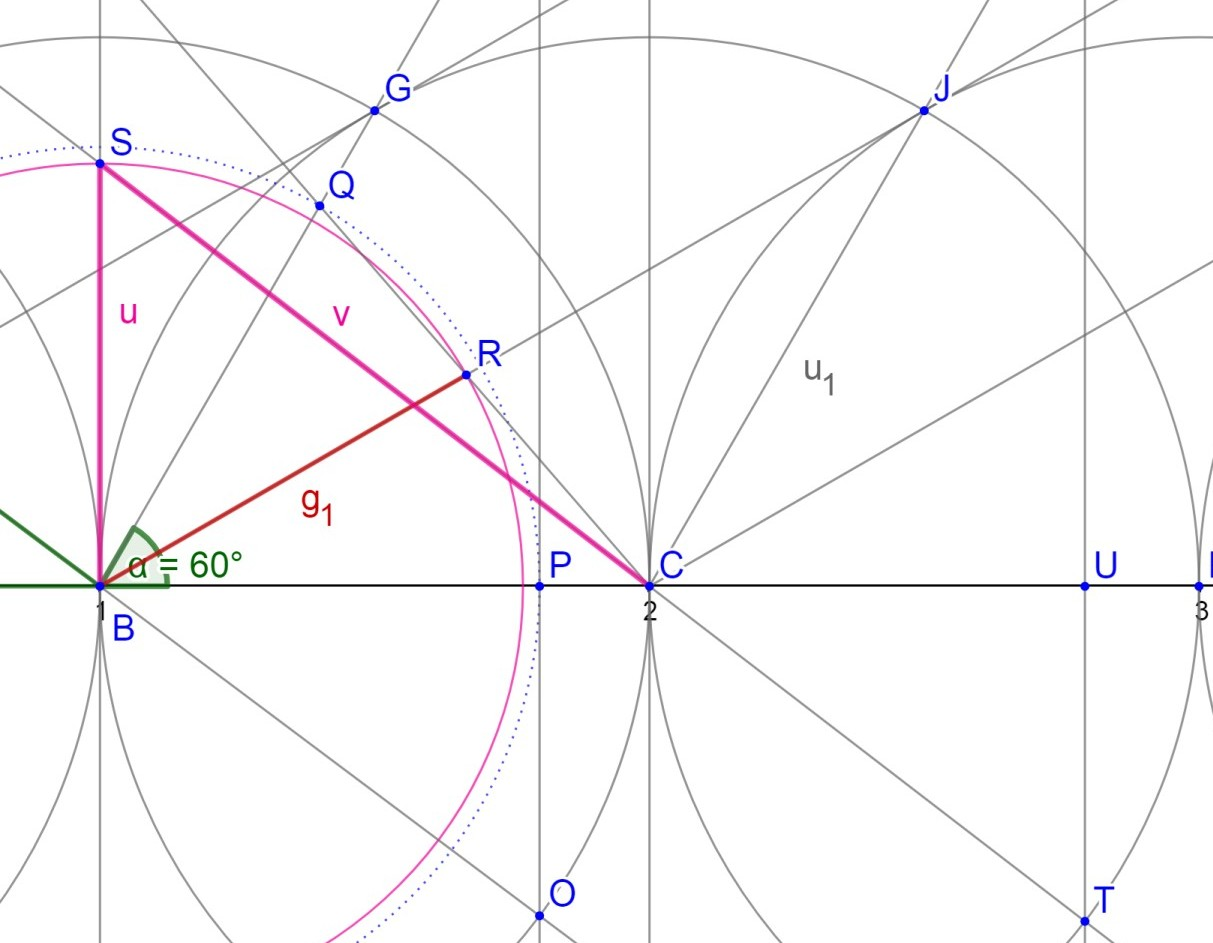
\includegraphics[scale=1]{triangle2.jpg}}
	\caption{Triangle BSC}
	\label{triangle_2}
\end{figure}

	\item Now we will repeat all the steps from the step 3.\\
	$\bullet$ We draw a line through the points $S,C$ and get the point $T$, as the intersection of the line and the circle with center at the point $C(2,0)$. \\
	Hence:
\begin{equation}
	 \dfrac{\overline{SC}}{\overline{BC}}=\overline{CU}= \cos \angle BCS
\end{equation}

$\bullet$ Then repeat the steps: 4, 5, 6, 7, 8 and repeat again from 3-rd step to the 8 step; and so on...\\
	\item Iterating it over and over we obtain $\sqrt[3]{2}$ as the length of the hypotenuse of the right triangle.
\begin{figure*}[h]
	\centering
	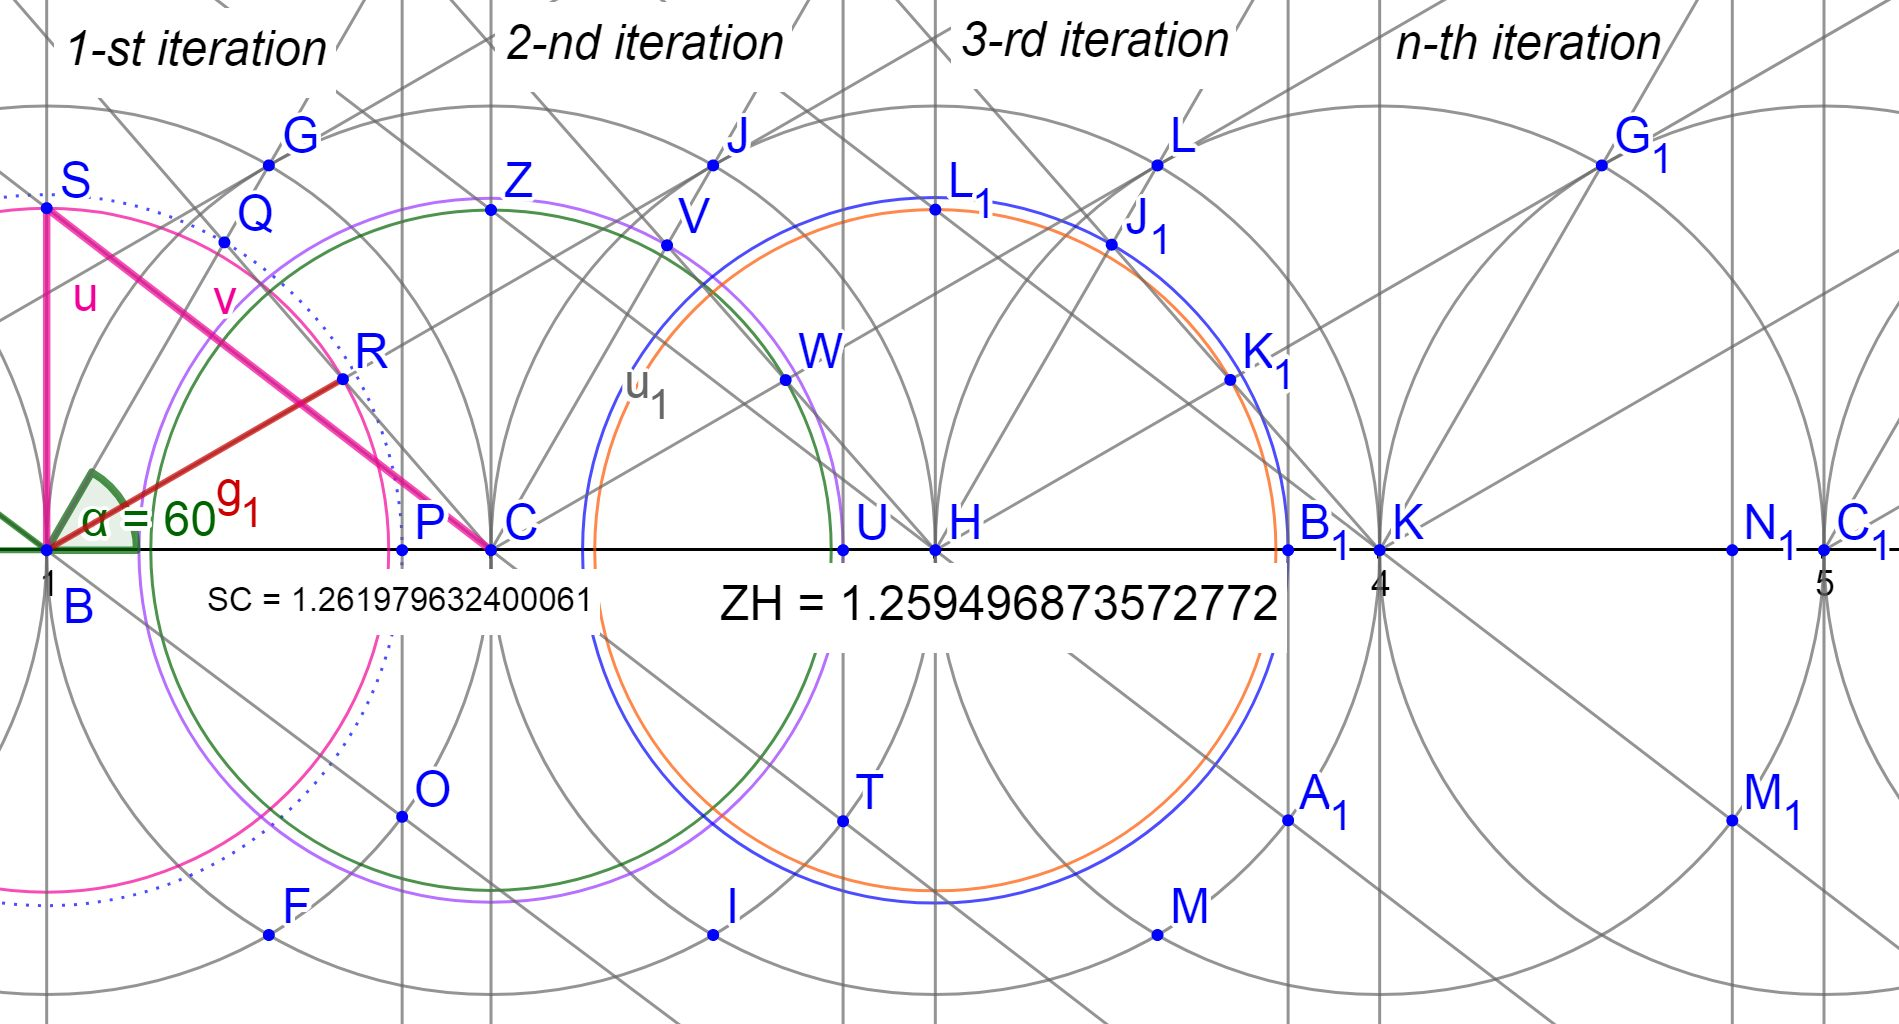
\includegraphics[width=0.7\linewidth]{iterations.jpg}
	\caption{Construction}
	\label{construction}
\end{figure*}
\end{enumerate}.

\newpage

\subsection{Proof} 


The main idea is similar to the recursion concept. 
%We recursively calculate \textit{$hypotenuse => cosine => bisector => hypotenuse => cosine => bisector => hypotenuse...$ and so on.}\\
The algorithm is looks like this:
\begin{enumerate}
\item[1] iteration:
\begin{equation}
\dfrac{1}{\sqrt{a^{2}+t_{0}^{2}}}=t_{1};\ \hspace{5pt} \frac{2\times t_{1}}{1+t_{1}}\times\frac{\sqrt{3}}{2}=t_{2}
\end{equation}
\item[2] iteration
\begin{equation}
 \dfrac{1}{\sqrt{a^{2}+t_{2}^{2}}}=t_{3};\ \hspace{5pt} \frac{2\times t_{3}}{1+t_{3}}\times\frac{\sqrt{3}}{2}=t_{4} \ ...
\end{equation}
\subitem n-th iteration:
\begin{equation}
\dfrac{1}{\sqrt{a^{2}+t_{n}^{2}}}=t_{n+1};\ \hspace{5pt} \frac{2\times t_{n+1}}{1+t_{n+1}}\times\frac{\sqrt{3}}{2}=t_{n+2} \ \hspace{5pt} ...
\end{equation}
\end{enumerate}
Where $t_{0}=t=0.75$ (see Figure \ref{fig:basic}). The shortest leg of the first right triangle is 0.75 since this value is easy to construct by a compass and unmarked straightedge.
However, we will get a cube root of 2, regardless of the length of the shortest leg at the beginning! The only rule is that the longest leg  should be equal to 1.
\\ 
After n-th iterations we get the length of the hypotenuse $s$
 $\approx\sqrt[3]{2}$. The accuracy depends on the number of iterations.\\ 
\begin{enumerate}

\item[1] iteration: $\triangle ANB$; (Figure \ref{fig:basic}) where $\overline{AN}=t=0.75$; therefore hypotenuse and cosine respectively:
\begin{equation}
 \overline{NB}=\sqrt{1^{2}+0.75^{2}}=1.25
 \end{equation}

\begin{equation}
\cos=\dfrac{1}{1.25}=0.8
\end{equation}

the length of the bisector:
\begin{equation}
 \frac{2\times0.8}{1+0.8}\times\frac{\sqrt{3}}{2}\approx 0.769800358919501
\end{equation}
\\
hypotenuse:
\begin{equation}
\sqrt{1^{2}+0,769800358919501^{2}}\approx 1,261979632400061
\end{equation}
\item[2] iteration:
%\textit{2-nd iteration} 
\begin{equation}
\cos=\dfrac{1}{1,261979632400061}\approx0,792405815693061
\end{equation}
bisector:
\begin{equation}
\frac{2\times 0.792405815693061}{1+0.792405815693061}\times\frac{\sqrt{3}}{2}\approx 0.765723432147395
\end{equation}
\\
Hypotenuse:
\begin{equation}
\sqrt{1^{2}+0.765723432147395^{2}}\approx 1.259496873572772
\end{equation}
\end{enumerate}
For convenience, I made calculations for 20 triangles, then imported the data into the table and analyzed the values.
\newpage
The table \ref{iterations and values} shows the calculated values of the bisector and hypotenuse, except for the cosine.
\\
\vspace{10pt}
%The last value of the hypotenuse is \textbf{1.259921049894873}, which is equal to  $\sqrt[3]{2}$ with an accuracy of $10^{-15}$. \\


\begin{tabular}{|c|c|c|} \hline
\centering
\textbf{iteration}	& \textbf{shortest leg=bisector} & \textbf{hypotenuse}\\	\hline
	$1$         & $0.769800358919501$ & $1.261979632400061$ \\ \hline
	$2$         & $0.765723432147395$ & $1.259496873572772$ \\ \hline
	$3$         & $0.766564817073686$ & $1.260008578849848$ \\ \hline
	$4$         & $0.766391253457252$ & $1.259902993637120$ \\ \hline
	$5$         & $0.766427060119643$ & $1.259924774930487$ \\ \hline
	$6$         & $0.766419673248706$ & $1.259920281423651$ \\ \hline
	$7$         & $0.766421197157344$ & $1.259921208430153$ \\ \hline
	$8$         & $0.766420882775838$ & $1.259921017189131$ \\ \hline
	$9$        & $0.76642094763258$ & $1.259921056642051$ \\ \hline
	$10$        & $0.766420934252668$ & $1.259921048502934$ \\ \hline
	$11$        & $0.766420937012937$ & $1.259921050182029$ \\ \hline
	$12$        & $0.766420936443495$ & $1.259921049835633$ \\ \hline
	$13$        & $0.76642093656097$ & $1.259921049907094$ \\ \hline
	$14$        & $0.766420936536735$ & $1.259921049892352$ \\ \hline
	$15$        & $0.766420936541735$ & $1.259921049895393$ \\ \hline
	$16$        & $0.766420936540704$ & $1.259921049894766$ \\ \hline
	$17$        & $0.766420936540916$ & $1.259921049894895$ \\ \hline
	$18$        & $0.766420936540872$ & $1.259921049894869$ \\ \hline
	$19$        & $0.766420936540881$ & $1.259921049894874$ \\ \hline
	$20$        & $0.766420936540879$ & $1.259921049894873$ \\ \hline

\end{tabular} 
\begin{table}[H] %due to the strange bug with table, here the trick; so that we can see a label and a caption for the table above 
	\caption {Iterations and values}
	\label{iterations and values}
\end{table}

Cubic equation obtained after plotting the values\footnote{I used geogebra.org/classic web app for plotting and analasis } in column B and applying polynominal regression model to the power of 3:
\begin{equation}
y=0.375x^{3}-0.5x^{2}+1.25x
\end{equation}
\begin{figure}[h]
	\centering
	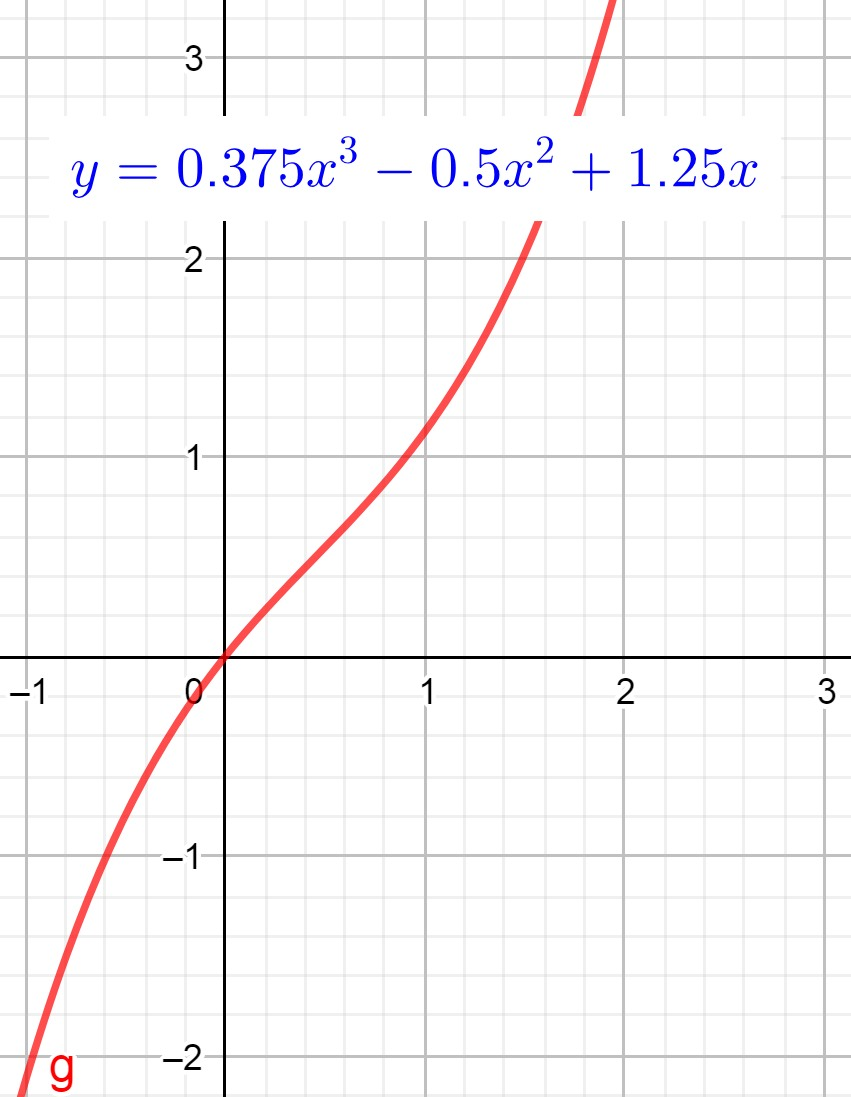
\includegraphics[width=0.2\linewidth]{g_x_func.jpg}
	\caption{Function}
	\label{fig:function}
\end{figure}\\
\newpage
We see that the value in column B on the 20th row (Table   \ref{iterations and values}) and the median value (see Figure \ref{fig:data}) is:  \textbf{1.259921049894873} = $\sqrt[3]{2}$ with an accuracy of $10^{-15}$.
\vspace{10pt}
\\
\begin{center}
	Reference value of the $\sqrt[3]{2}$ = \textbf{1.25992104989487316…} (rounded to 17th decimal place)
\end{center}
\vspace{10pt}
%\vfill in the beginning we can take any arbitrary length as the shortest leg of the right triangle.\\ For convenience, it is better to use a length equal to 0.75, which is easy to construct with compass and straightedge.\\


%\section{Theorem} TODO
%Diamond section is the way to find the hypotenuse of the right triangle with longest leg equal to 1, so that cosine of the angle between longest leg and hypotenuse ... 


During calculations I used rounding to the  $10^{-15}$, however we can get the final value with any given accuracy. This is because the length of the longest side tend to the cube root of two.
\\
\begin{figure}[h]
	\centering
	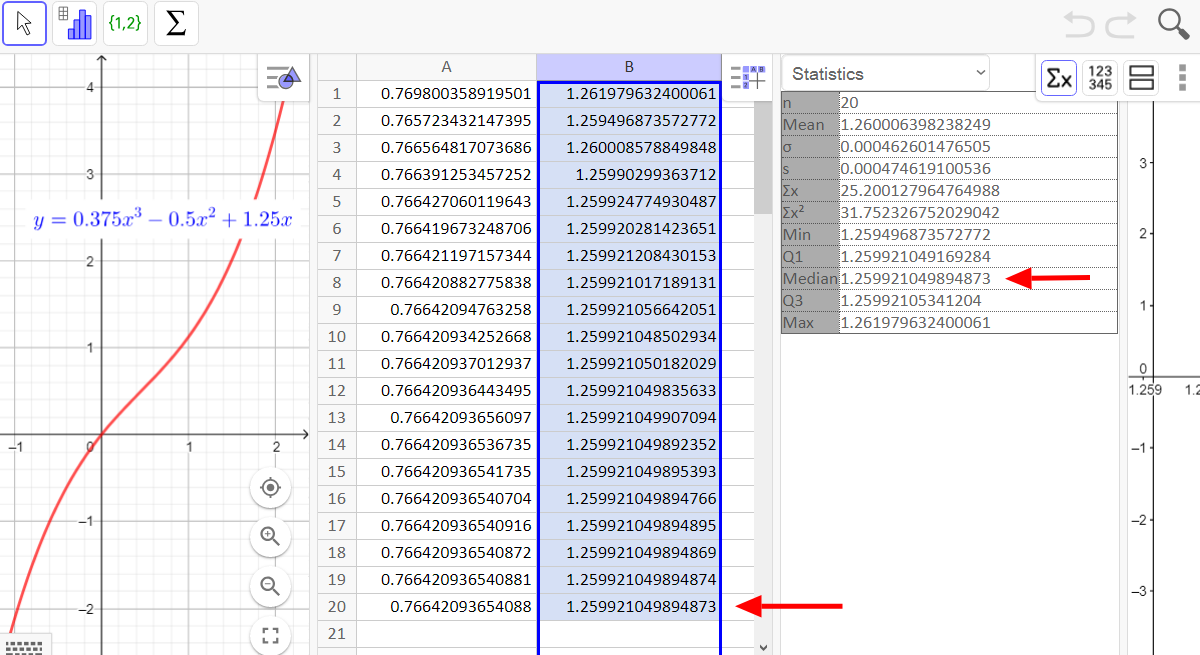
\includegraphics[width=0.9\linewidth]{Table_arrow.png}
	\caption{Data analysis}
	\label{fig:data}
\end{figure}
\begin{figure}[h]
	\centering
	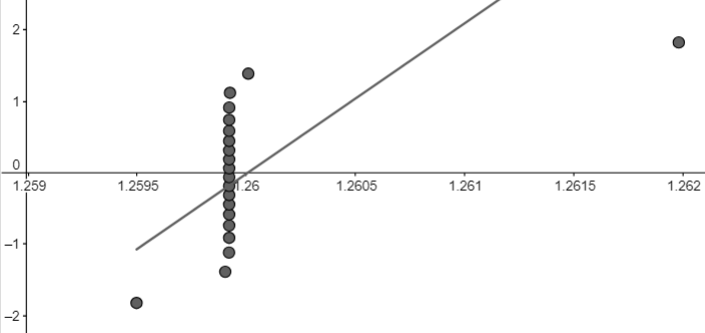
\includegraphics[width=0.9\linewidth]{plot.png}
	\caption{Normal Quantile plot}
	\label{fig:plot}
\end{figure}
\newpage

\section{Definition}

For the given right triangle $\triangle ABS$ with longest leg $a=1$ and  the bisector $g$ of $\angle SAY=60\degree$ (see Figure \ref{fig:definition}) the Diamond section is the condition where:
\begin{equation}
d=\frac{a}{s}=\frac{1}{\sqrt{1+b^{2}}}
\end{equation}
\\
\begin{equation}
 g=\frac{2\times d}{1+d}\times\frac{\sqrt{3}}{2}
\end{equation}
\\
\begin{equation}
b=g
\end{equation}
\\
\begin{equation}
s=\dfrac{1}{d}=\sqrt[3]{2}
\end{equation}
\\
\begin{figure}[h]
	\centering
	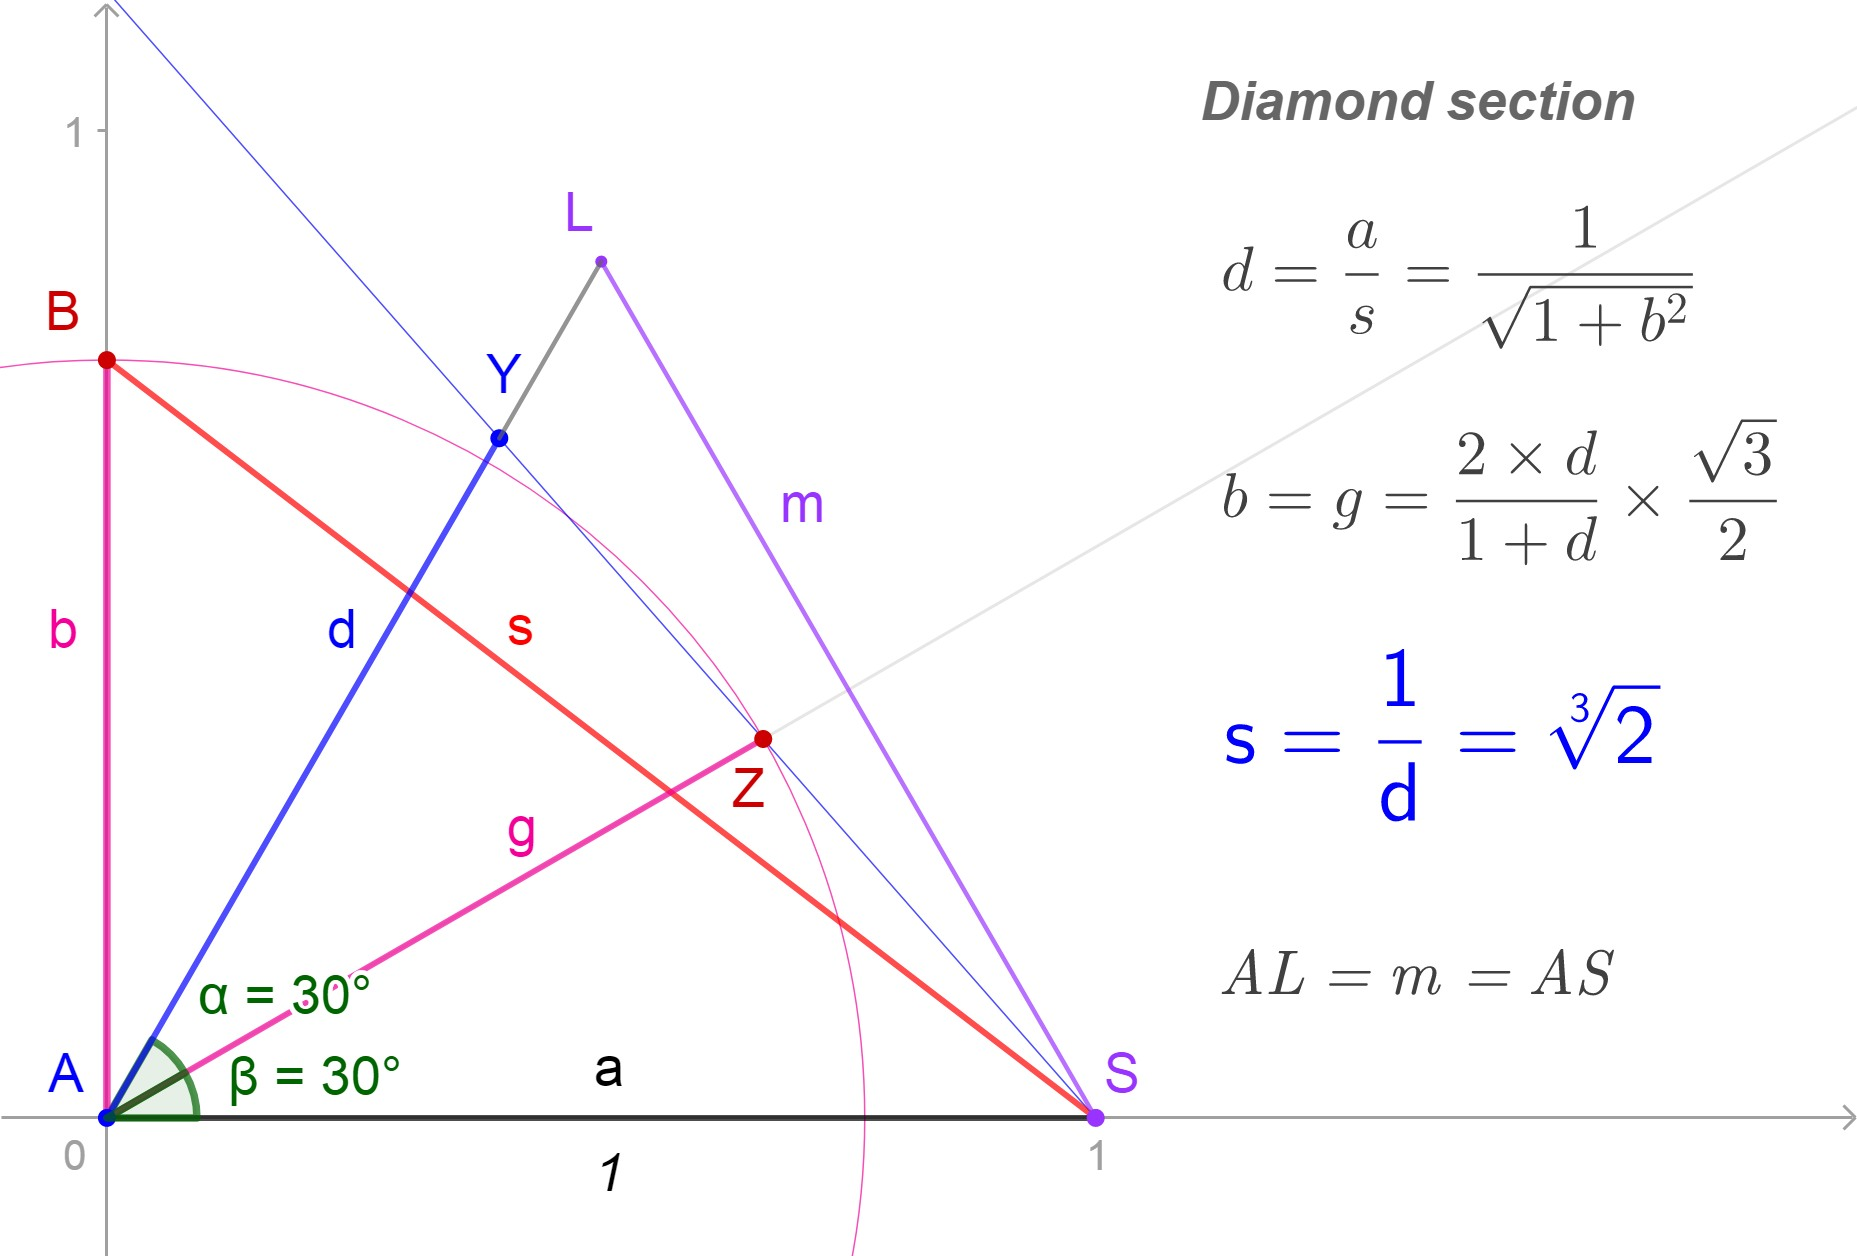
\includegraphics[width=0.7\linewidth]{ds_new_def.jpg}
	\caption{Definition}
	\label{fig:definition}
\end{figure} \\

\begin{center}
	\large{Diamond section of  $60 \degree$ angle = $\sqrt[3]{2}$ }
\\
%\begin{equation}
%$\sqrt[3]{2}=\lim_{ n \to \infty } \sqrt{1^{2}+b_{n}^{2}}$; $b_{1}>0$; 
%\end{equation} 
%$\sqrt[3]{2}=\lim_{ n \to \infty\frac{1}s_{n}}$
\end{center}
\newpage
 
\section {Why}
A diamond is a crystall of tetrahedrally bonded carbon atoms.
Each carbon atom in the diamond structure is located at the center of the tetrahedron, whose vertices are the four nearest atoms.\cite{B}
\\
The orthogonal vertex projection of a tetrahedron on a 2-D plane is a triangle. (Figure \ref{fig:tetrahedron}).
\begin{figure}[h]
	\centering
	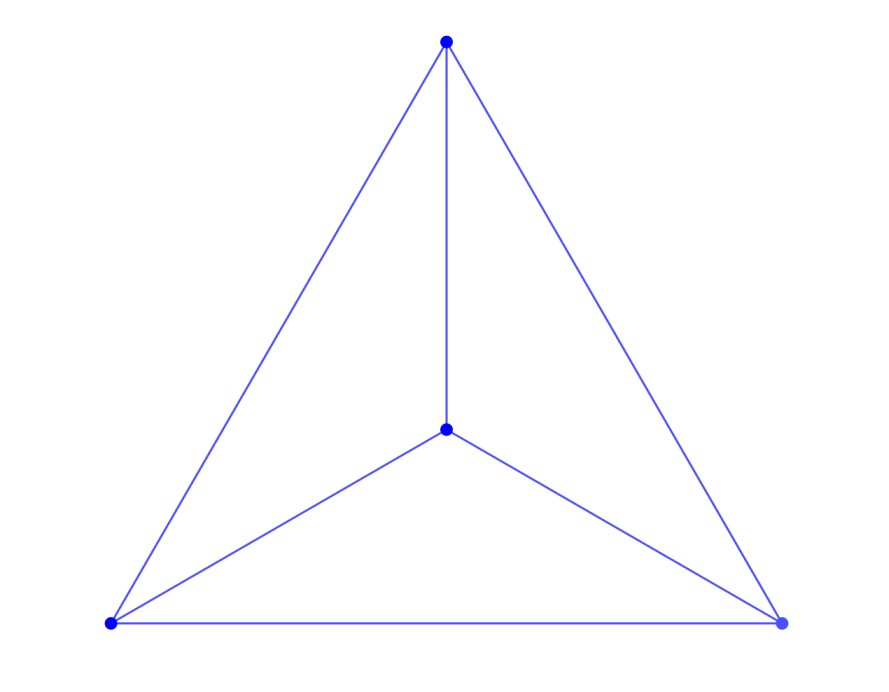
\includegraphics[width=0.3\linewidth]{tetrahedron}
	\caption{Vertex projection of tetrahedron}
	\label{fig:tetrahedron}
\end{figure}


\section{Conclusion}
\begin{center}
	Eventually, 2000 years later, the problem is solved, and the \textbf{cube root of two} \textbf{can be constructed} by a compass and unmarked straightedge.
\end{center}



\begin{figure}[h]
	\centering
	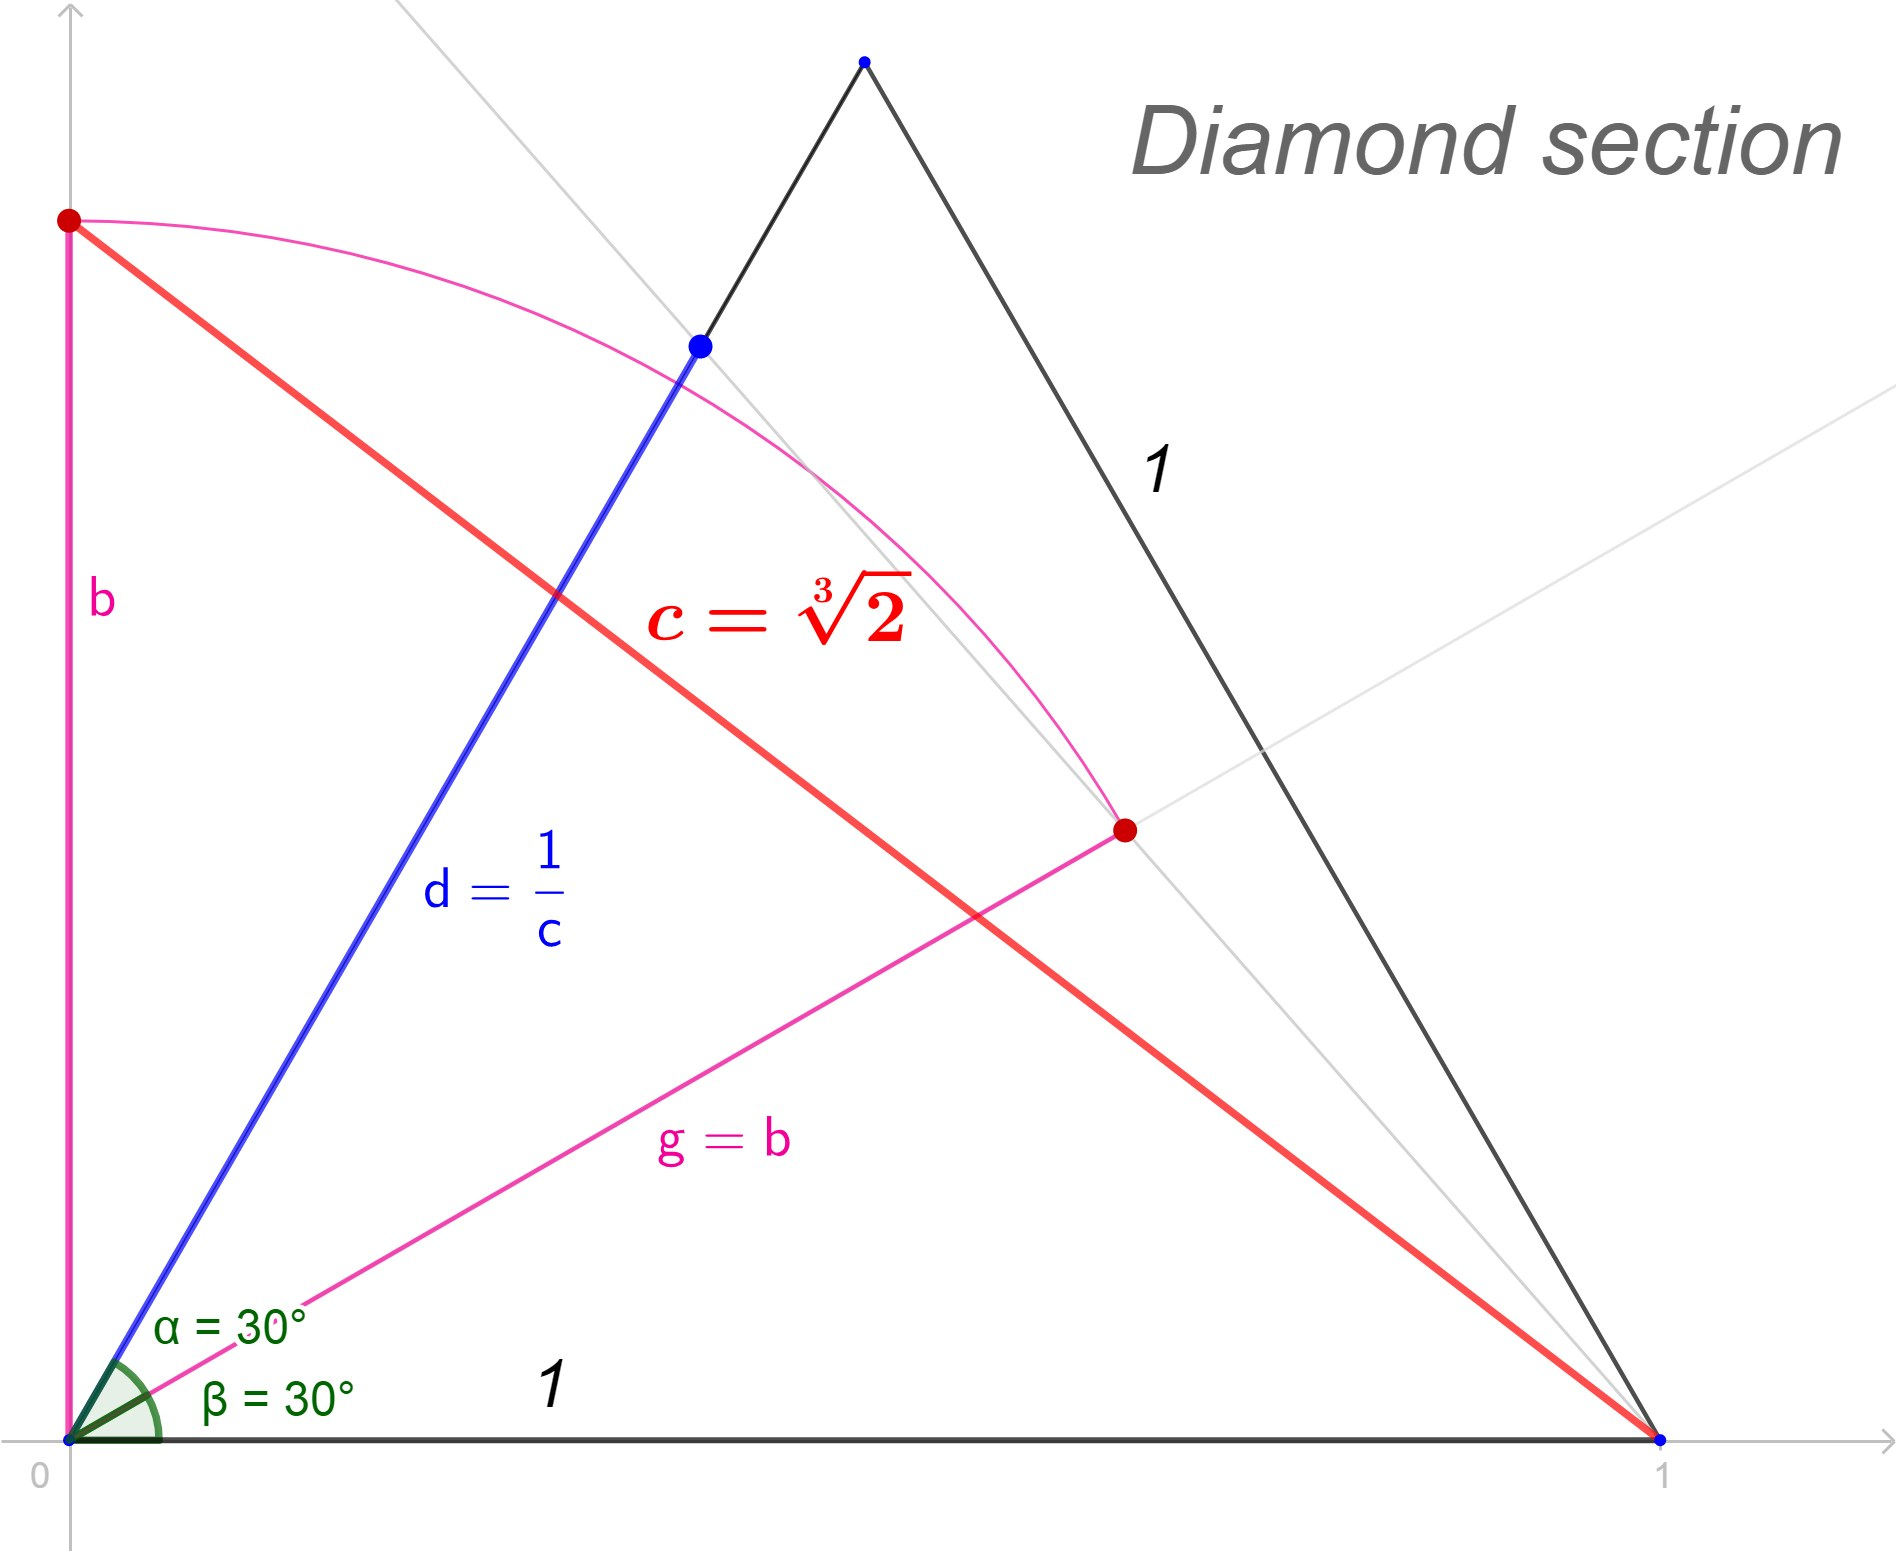
\includegraphics[width=0.6\linewidth]{ds_def.jpg}
	
	\label{fig:Diamond Section}
\end{figure}

\newpage

\section{Appendix}

I found an interesting property of the right triangle with sides: $a=1$; $b=\sqrt{\varphi-1}$; $c=\sqrt{\varphi}$\\
where $\varphi\approx 1.6180339887$ (see Figure \ref{fig:mytriangle})
\begin{figure}[h]
	\centering
	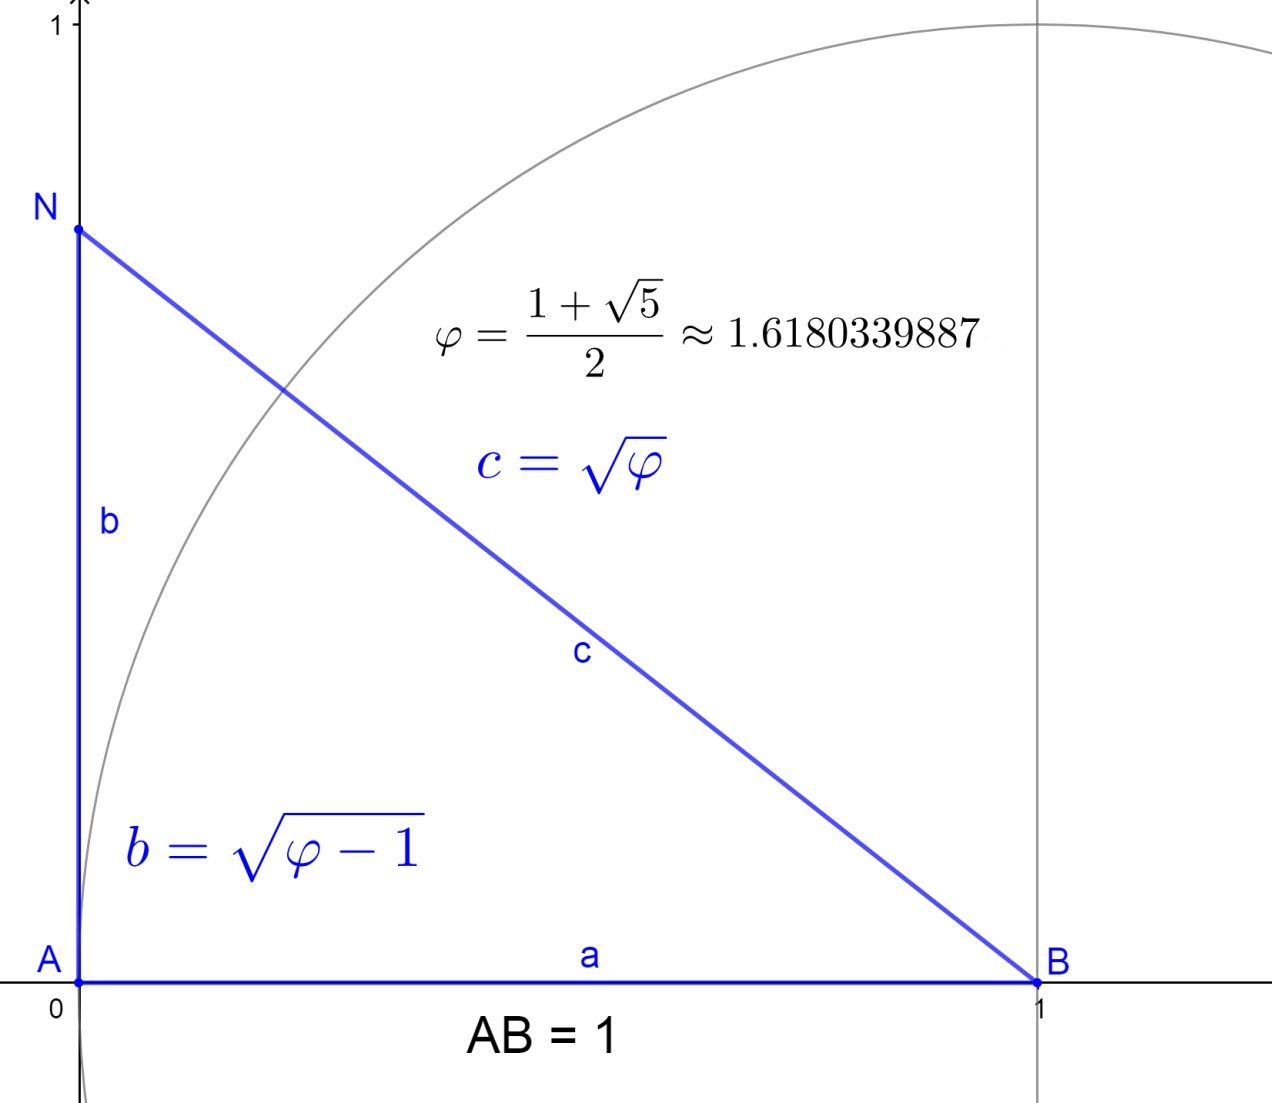
\includegraphics[width=0.7\linewidth]{my_triangle.jpg}
	\caption{Interesting triangle}
	\label{fig:mytriangle}
\end{figure}

If we take an \textbf{arbitrary} length as the shortest leg $b$ of the right triangle with longest leg $a=1$, and recursively apply this:
\begin{equation}
\dfrac{1}{\sqrt{a^2+b^2}} = b_{1}; \   \dfrac{1}{\sqrt{a^2+b_{1}^2}} = b_{2}; \   \dfrac{1}{\sqrt{a^2+b_{2}^2}}=b_{3}; \ ... \dfrac{1}{\sqrt{a^2+b_{n-1}^2}}=b_{n}
\end{equation} 
Then, after the n-th iteration\footnote{The accuracy depends on the number of iterations.} we get:
\begin{equation}
a=1;
\end{equation}
\\
\begin{equation}
b=\sqrt{\varphi-1}
\end{equation}
\\
\begin{equation}
c=\sqrt{\varphi}
\end{equation}
Therefore, our triangle with an arbitrary shortest leg became to the triangle shown in the Figure \ref{fig:mytriangle}.
\\
In other words the shortest leg $b$ tend to $\sqrt{\varphi-1}$
\\
%Definition: \\
%\begin{equation}
%\sqrt{\varphi-1}=\lim_{n\to\infty}\dfrac{1}{d_{n}}; \      b>0; \   
%d_{1}=\dfrac{1}{\sqrt{1^{2}+b^{2}}}; \  \    %d_{2}=\dfrac{1}{\sqrt{{1^2+d_{1}^2}}}; \  ...\ %d_{n}=\dfrac{1}{\sqrt{{1^2+d_{n-1}^2}}}
%\end{equation}
%\begin{equation}
%\sqrt{\varphi}=\lim_{n\to\infty}\sqrt{d_{n}^2+1}; \      b>0; \   
%d_{1}=\dfrac{1}{\sqrt{1^{2}+b^{2}}}; \  \    %d_{2}=\dfrac{1}{d_{1}}; \  ...\ %d_{n}=\dfrac{1}{d_{n-1}};
%\end{equation}

%TODO: To construct the $\pi$ by using a compass and straightedge.\\
%next time 
 
\newpage


\begin{minipage}{0.8\textwidth}

\title{text}

	
\section{Resources}

%\large \textbf{Author:}

website: \url{ http://diamondsection.com} \\
e-mail: jobspace@yandex.com \\
github: \url{https://github.com/AlmasAskarbekov}

\section{Thanks}
\url{https://geogebra.org}
\\
\section{Notes}
Note: I used a standard calculator built into the operating system to get the values from the spreadsheet (Table \ref{iterations and values} 1.6). The geogebra web application uses javascript, which means that if I used a web application to calculate all the values measuring the length between two points, I would get a slightly different value. This is due to how javascript stores floating point numbers\cite{C}.  However, in the end we get the cube root of two in any case, because the length of the longest side tends to the cube root of two.
\end{minipage}
\vspace{365pt}
\hrule
\ 
\\
\emph{Keywords: Geometric problems of Antiquity, geometry, doubling the cube, the delians problem}




\begin{thebibliography}{5}
\bibitem{A}
\url{https://en.wikipedia.org/wiki/Doubling_the_cube}
\bibitem{B}
\url{https://en.wikipedia.org/wiki/Diamond}
\bibitem{C}
\url{https://en.wikipedia.org/wiki/IEEE_754}
\end{thebibliography}

\vspace{465pt}
@misc{DiamondSection2018,
	author = {Almas Askarbekov},
	title = {Doubling the cube. Solution},
	year = {2018},
	howpublished = {\url{https://github.com/DiamondSection/Doubling-the-cube-Solution_Latex}},
	note = {commit dbgsxxx}
}
%%%%%%Dedicated to Delos%%%%%%%% 
\end{document}